% GNUPLOT: LaTeX picture with Postscript
\begingroup
\footnotesize
  \makeatletter
  \providecommand\color[2][]{%
    \GenericError{(gnuplot) \space\space\space\@spaces}{%
      Package color not loaded in conjunction with
      terminal option `colourtext'%
    }{See the gnuplot documentation for explanation.%
    }{Either use 'blacktext' in gnuplot or load the package
      color.sty in LaTeX.}%
    \renewcommand\color[2][]{}%
  }%
  \providecommand\includegraphics[2][]{%
    \GenericError{(gnuplot) \space\space\space\@spaces}{%
      Package graphicx or graphics not loaded%
    }{See the gnuplot documentation for explanation.%
    }{The gnuplot epslatex terminal needs graphicx.sty or graphics.sty.}%
    \renewcommand\includegraphics[2][]{}%
  }%
  \providecommand\rotatebox[2]{#2}%
  \@ifundefined{ifGPcolor}{%
    \newif\ifGPcolor
    \GPcolortrue
  }{}%
  \@ifundefined{ifGPblacktext}{%
    \newif\ifGPblacktext
    \GPblacktexttrue
  }{}%
  % define a \g@addto@macro without @ in the name:
  \let\gplgaddtomacro\g@addto@macro
  % define empty templates for all commands taking text:
  \gdef\gplbacktext{}%
  \gdef\gplfronttext{}%
  \makeatother
  \ifGPblacktext
    % no textcolor at all
    \def\colorrgb#1{}%
    \def\colorgray#1{}%
  \else
    % gray or color?
    \ifGPcolor
      \def\colorrgb#1{\color[rgb]{#1}}%
      \def\colorgray#1{\color[gray]{#1}}%
      \expandafter\def\csname LTw\endcsname{\color{white}}%
      \expandafter\def\csname LTb\endcsname{\color{black}}%
      \expandafter\def\csname LTa\endcsname{\color{black}}%
      \expandafter\def\csname LT0\endcsname{\color[rgb]{1,0,0}}%
      \expandafter\def\csname LT1\endcsname{\color[rgb]{0,1,0}}%
      \expandafter\def\csname LT2\endcsname{\color[rgb]{0,0,1}}%
      \expandafter\def\csname LT3\endcsname{\color[rgb]{1,0,1}}%
      \expandafter\def\csname LT4\endcsname{\color[rgb]{0,1,1}}%
      \expandafter\def\csname LT5\endcsname{\color[rgb]{1,1,0}}%
      \expandafter\def\csname LT6\endcsname{\color[rgb]{0,0,0}}%
      \expandafter\def\csname LT7\endcsname{\color[rgb]{1,0.3,0}}%
      \expandafter\def\csname LT8\endcsname{\color[rgb]{0.5,0.5,0.5}}%
    \else
      % gray
      \def\colorrgb#1{\color{black}}%
      \def\colorgray#1{\color[gray]{#1}}%
      \expandafter\def\csname LTw\endcsname{\color{white}}%
      \expandafter\def\csname LTb\endcsname{\color{black}}%
      \expandafter\def\csname LTa\endcsname{\color{black}}%
      \expandafter\def\csname LT0\endcsname{\color{black}}%
      \expandafter\def\csname LT1\endcsname{\color{black}}%
      \expandafter\def\csname LT2\endcsname{\color{black}}%
      \expandafter\def\csname LT3\endcsname{\color{black}}%
      \expandafter\def\csname LT4\endcsname{\color{black}}%
      \expandafter\def\csname LT5\endcsname{\color{black}}%
      \expandafter\def\csname LT6\endcsname{\color{black}}%
      \expandafter\def\csname LT7\endcsname{\color{black}}%
      \expandafter\def\csname LT8\endcsname{\color{black}}%
    \fi
  \fi
    \setlength{\unitlength}{0.0500bp}%
    \ifx\gptboxheight\undefined%
      \newlength{\gptboxheight}%
      \newlength{\gptboxwidth}%
      \newsavebox{\gptboxtext}%
    \fi%
    \setlength{\fboxrule}{0.5pt}%
    \setlength{\fboxsep}{1pt}%
\begin{picture}(6780.00,5080.00)%
    \gplgaddtomacro\gplbacktext{%
      \csname LTb\endcsname%%
      \put(566,3429){\makebox(0,0)[r]{\strut{}$0$}}%
      \csname LTb\endcsname%%
      \put(566,3657){\makebox(0,0)[r]{\strut{}$0.2$}}%
      \csname LTb\endcsname%%
      \put(566,3886){\makebox(0,0)[r]{\strut{}$0.4$}}%
      \csname LTb\endcsname%%
      \put(566,4114){\makebox(0,0)[r]{\strut{}$0.6$}}%
      \csname LTb\endcsname%%
      \put(566,4343){\makebox(0,0)[r]{\strut{}$0.8$}}%
      \csname LTb\endcsname%%
      \put(566,4571){\makebox(0,0)[r]{\strut{}$1$}}%
      \csname LTb\endcsname%%
      \put(678,3225){\makebox(0,0){\strut{}$0$}}%
      \csname LTb\endcsname%%
      \put(1074,3225){\makebox(0,0){\strut{}$50$}}%
      \csname LTb\endcsname%%
      \put(1470,3225){\makebox(0,0){\strut{}$100$}}%
      \csname LTb\endcsname%%
      \put(1867,3225){\makebox(0,0){\strut{}$150$}}%
      \csname LTb\endcsname%%
      \put(2263,3225){\makebox(0,0){\strut{}$200$}}%
    }%
    \gplgaddtomacro\gplfronttext{%
      \csname LTb\endcsname%%
      \put(44,4000){\rotatebox{-270}{\makebox(0,0){\strut{}Fraction of expr.}}}%
      \csname LTb\endcsname%%
      \put(1660,2919){\makebox(0,0){\strut{}Generations}}%
      \csname LTb\endcsname%%
      \put(1660,4877){\makebox(0,0){\strut{}Len=10, Pop=100}}%
    }%
    \gplgaddtomacro\gplbacktext{%
      \csname LTb\endcsname%%
      \put(2712,3225){\makebox(0,0){\strut{}$0$}}%
      \csname LTb\endcsname%%
      \put(3108,3225){\makebox(0,0){\strut{}$50$}}%
      \csname LTb\endcsname%%
      \put(3504,3225){\makebox(0,0){\strut{}$100$}}%
      \csname LTb\endcsname%%
      \put(3901,3225){\makebox(0,0){\strut{}$150$}}%
      \csname LTb\endcsname%%
      \put(4297,3225){\makebox(0,0){\strut{}$200$}}%
    }%
    \gplgaddtomacro\gplfronttext{%
      \csname LTb\endcsname%%
      \put(3694,2919){\makebox(0,0){\strut{}Generations}}%
      \csname LTb\endcsname%%
      \put(3694,4877){\makebox(0,0){\strut{}Len=12, Pop=100}}%
    }%
    \gplgaddtomacro\gplbacktext{%
      \csname LTb\endcsname%%
      \put(4746,3225){\makebox(0,0){\strut{}$0$}}%
      \csname LTb\endcsname%%
      \put(5142,3225){\makebox(0,0){\strut{}$50$}}%
      \csname LTb\endcsname%%
      \put(5538,3225){\makebox(0,0){\strut{}$100$}}%
      \csname LTb\endcsname%%
      \put(5935,3225){\makebox(0,0){\strut{}$150$}}%
      \csname LTb\endcsname%%
      \put(6331,3225){\makebox(0,0){\strut{}$200$}}%
    }%
    \gplgaddtomacro\gplfronttext{%
      \csname LTb\endcsname%%
      \put(5728,2919){\makebox(0,0){\strut{}Generations}}%
      \csname LTb\endcsname%%
      \put(5728,4877){\makebox(0,0){\strut{}Len=20, Pop=500}}%
      \csname LTb\endcsname%%
      \put(2637,610){\makebox(0,0)[r]{\strut{}distinct expr}}%
      \csname LTb\endcsname%%
      \put(2637,406){\makebox(0,0)[r]{\strut{}distinct structures}}%
      \csname LTb\endcsname%%
      \put(5854,610){\makebox(0,0)[r]{\strut{}distinct structures (simplified)}}%
      \csname LTb\endcsname%%
      \put(5854,406){\makebox(0,0)[r]{\strut{}p1 evaluations}}%
    }%
    \gplgaddtomacro\gplbacktext{%
      \csname LTb\endcsname%%
      \put(566,1524){\makebox(0,0)[r]{\strut{}$0$}}%
      \csname LTb\endcsname%%
      \put(566,1752){\makebox(0,0)[r]{\strut{}$0.2$}}%
      \csname LTb\endcsname%%
      \put(566,1981){\makebox(0,0)[r]{\strut{}$0.4$}}%
      \csname LTb\endcsname%%
      \put(566,2209){\makebox(0,0)[r]{\strut{}$0.6$}}%
      \csname LTb\endcsname%%
      \put(566,2438){\makebox(0,0)[r]{\strut{}$0.8$}}%
      \csname LTb\endcsname%%
      \put(566,2666){\makebox(0,0)[r]{\strut{}$1$}}%
      \csname LTb\endcsname%%
      \put(1071,1320){\makebox(0,0){\strut{}$5000$}}%
      \csname LTb\endcsname%%
      \put(1857,1320){\makebox(0,0){\strut{}$15000$}}%
    }%
    \gplgaddtomacro\gplfronttext{%
      \csname LTb\endcsname%%
      \put(44,2095){\rotatebox{-270}{\makebox(0,0){\strut{}Fraction of evals.}}}%
      \csname LTb\endcsname%%
      \put(1660,1014){\makebox(0,0){\strut{}Evaluations}}%
    }%
    \gplgaddtomacro\gplbacktext{%
      \csname LTb\endcsname%%
      \put(3105,1320){\makebox(0,0){\strut{}$5000$}}%
      \csname LTb\endcsname%%
      \put(3891,1320){\makebox(0,0){\strut{}$15000$}}%
    }%
    \gplgaddtomacro\gplfronttext{%
      \csname LTb\endcsname%%
      \put(3694,1014){\makebox(0,0){\strut{}Evaluations}}%
    }%
    \gplgaddtomacro\gplbacktext{%
      \csname LTb\endcsname%%
      \put(4825,1320){\makebox(0,0){\strut{}$5000$}}%
      \csname LTb\endcsname%%
      \put(5611,1320){\makebox(0,0){\strut{}$55000$}}%
    }%
    \gplgaddtomacro\gplfronttext{%
      \csname LTb\endcsname%%
      \put(5728,1014){\makebox(0,0){\strut{}Evaluations}}%
    }%
    \gplbacktext
    \put(0,0){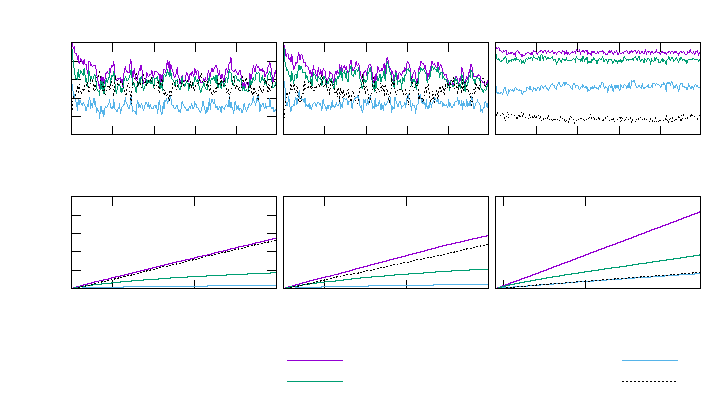
\includegraphics{../plots/nikuradse_2_run1_uniq}}%
    \gplfronttext
  \end{picture}%
\endgroup
